\appendix 
\chapter{Omitted Proofs}
\label{chap:app}

\section{Chapter~\ref{chap:background}}
\label{sec:app_proofs_background}


\begin{proof}[Proof  of  Observation~\ref{obs:bi-orthogonal_unique}]
	We begin by  proving uniqueness. 
	Suppose $\{\u_i\}$ and $\{\w_i\}$ are both biorthogonal bases of $\{\v_i\}$. We will show that $\u_i=\w_i$  for all $i$. Fix $i\in[n]$. By independence, $\spn(\v_1,\dots,\v_{i-1},\v_{i+1},\dots,\v_n)$ is a hyperplane---that is, \[\dim\spn(\v_1,\dots,\v_{i-1},\v_{i+1},\dots,\v_n)^\perp=1.\] (Recall  that we are  working in $\R^n$ and with bases thereof.) Both $\u_i$ and $\w_i$ are orthogonal to this hyperplane (since they orthogonal to $\v_j$ for all $j\neq i$), thus are either parallel or anti-parallel. Therefore, there exists some $\alpha\in\R$ such that $\v_i=\alpha\w_i$. By definition, $\la \v_i,\u_i\ra = \la \v_i,\w_i\ra =1$, hence $\la \v_i,\alpha \w_i\ra = \la \v_i,\w_i\ra$ implying that $\alpha=1$. This demonstrates that $\u_i=\w_i$ for all $i$. 
	
	Next we demonstrate that  $\Q^\tp=\M^{-1}$ where $\Q=(\u_1,\dots,\u_n)$ and $\M=(\v_1,\dots,\v_n)$. By the orthogonality relationships of dual bases, we have  
	\[\Q^\tp\M = \begin{pmatrix}
	\u_1^\tp \\
	\vdots  \\
	\u_n^\tp
	\end{pmatrix}
	\begin{pmatrix}
	\v_1 & \dots & \v_n
	\end{pmatrix} = \begin{pmatrix}
	\la \u_1,\v_1\ra & \dots & \la \u_1,\v_n \\
	\vdots & \ddots & \vdots  \\
	\la \u_n,\v_1\ra & \dots & \la \u_n,\v_n\ra 
	\end{pmatrix} = \I_n.
	\]
	Observing that $\M^{-1}$ exists by independence of $\{\v_1,\dots,\v_n\}$ we apply it  to  both sides of the  above to obtain   $\Q^\tp=\M^{-1}$. 
\end{proof}

\begin{proof}[Proof of Lemma~\ref{lem:rank(QtQ)}]
	It suffices to show that $\dim\ker\Q = \dim\ker\Q^\tp \Q$, by rank-nullity. Clearly $\ker\Q \subset \ker\Q^\tp\Q$ since $\Q\f=\zero$ implies $\Q^\tp\Q\f=\zero$. Conversely, if $\Q^\tp\Q\f=\zero$ then $0=\f^\tp \Q^\tp \Q\f = \norm{\Q\f}_2^2$, implying that $\Q\f=\zero$.  
\end{proof}

\begin{proof}[Proof of Lemma~\ref{lem:pseudoinverse_eigendecomposition}]
	Put $\vb{Q}=\sum_{i=1}^k \lambda_i^{-1}\vp_i\vp_I^\tp$. Since the pseudoinverse is unique, it suffices to show that $\vb{Q}$ satisfies the condition of Definition \ref{def:pseudoinverse}.
	Since the eigenvectors are orthonormal by assumption, $\vp_i^\tp\vp_j=\delta_{i,j}$ for all $i,j$. Hence,  
	\begin{align*}
	\M\vb{Q}&= \sum_{i=1}^k \lambda_i\vp_i\vp_i^\tp \sum_{j=1}^k \lambda_j^{-1}\vp_j\vp_j^\tp = \sum_{i,j=1}^k \lambda_i\lambda_j^{-1} \vp_i\vp_i^\tp \vp_j\vp_j^\tp \\
	&= \sum_{i=1}^k \lambda_i\lambda_i^{-1} \vp_i\vp_i^\tp\vp_i\vp_i^\tp 
	= \sum_{i=1}^k \vp_i\vp_i^\tp = \vb{Q}\M.
	\end{align*}
	Performing a similar computation then demonstrates that 
	\[\M\vb{Q}\M = \sum_{i=1}^k \vp_i\vp_i^\tp \sum_{j=1}^k \lambda_j\vp_j\vp_j^\tp=\sum_{i,j=1}\lambda_i \vp_i\vp_i^\tp\vp_j\vp_j^\tp=\sum_{i=1}^k \lambda_i \vp_i\vp_i^\tp =\M,\]
	and similarly, $\vb{Q}\M\vb{Q}=\vb{Q}$. Moreover, $\vp_i\vp_i^\tp (k,\ell)=\vp_i(k)\vp_i(\ell)=\vp_i(\ell)\vp_i(k)=(\vp_i\vp_i^\tp)^\tp (k,\ell)$ implying that $\vp_i\vp_i^\tp=(\vp_i\vp_i^\tp)^\tp$, so 
	\[(\vb{Q}\M)^\tp=(\M\vb{Q})^\tp =\bigg(\sum_{i=1}^k \vp_i\vp_i^\tp \bigg)^\tp = \sum_{i=1}^k (\vp_i\vp_i^\tp)^\tp = \sum_{i=1}^k \vp_i\vp_i^\tp=\M\vb{Q}=\vb{Q}\M,\]
	so both required conditions hold, and we conclude that $\vb{Q}=\M^+$. 
\end{proof}

\begin{proof}[Proof of Lemma~\ref{lem:er_props}]
	By definition 
	\begin{equation*}
	\Reff_G(i,j) = \bchi_i^\tp\L_G^+\bchi_i + \bchi_j^\tp \L_G^+\bchi_j -2 \bchi_i^\tp \L_G^+\bchi_j = \L_G^+(i,i) + \L_G^+(j,j) - 2\L_G^+(i,j),
	\end{equation*}
	whence
	\begin{equation*}
	\Reff_G = \one \u ^\tp + \u\one^\tp - 2\L_G^+,
	\end{equation*}
	(where we recall that  $\u=\diag(\L_G^+(i,i))$).  From here we  see that $\x^\tp \Reff_G\x = -2\x^\tp \L_G^+\x$ for any $\x\in\spn(\one)^\perp$. Therefore, 
	\begin{align}
	\L_G^+(i,j)&=\bchi_i^\tp \L_G^+\bchi_j \notag \\
	&= \bigg(\bchi_i-\frac{1}{n}\one\bigg)^\tp \L_G^+\bigg(\bchi_j-\frac{1}{n}\one\bigg) \notag \\
	&= -\frac{1}{2}\bigg(\bchi_i-\frac{1}{n}\one\bigg)^\tp \Reff_G\bigg(\bchi_j-\frac{1}{n}\one\bigg) \notag \\
	&= \frac{1}{2n}\bigg(\sum_{k\in[n]}\effr(i,k)+\effr(j,k)\bigg) - \frac{1}{2}\effr(i,j) -\frac{R_G}{n^2}.\notag\qedhere 
	\end{align}
\end{proof}

\begin{proof}[Proof of Lemma~\ref{lem:laplacian_props}]
	Focus for the moment on the combinatorial Laplacian  $\L_G$, with eigenvalues $\lambda_1\geq \lambda_2\geq \dots \geq \lambda_n$ and corresponding orthonormal eigenfunctions $\vp_1,\dots,\vp_n$. It is a straightforward consequence of Equation \eqref{eq:L=BTB} is that all eigenvalues of $\L_G$ are non-negative. Let $\lambda$ be an eigenvalue with (unit) eigenvector $\vp$. Then,  
	\begin{equation*}
	\lambda = \lambda\la \vp,\vp\ra = \la \lambda \vp,\vp\ra = \la \L_G\vp,\vp\ra = \la \B_G^\tp \B_G\vp,\vp\ra = \la \B_G\vp,\B_G\vp\ra =\norm{\B_G\vp}_2^2 \geq 0.
	\end{equation*}
	Now, suppose $\L\vp=\zero$. Then $\vp^\tp\L\vp=\Lf(\vp)=0$, which implies that $\vp(i)=\vp(j)$ for all $i,j\in V_\ell$. We can immediately see that any vector in $\spn(1)$ satisfies this condition. 
	On the other hand, consider a non-zero vector $\vp$ which is orthogonal to $\one$. Then 
	\[0=\sum_{i=1}^k \la \vp,\bchi_{V_i}\ra = \la \vp,\one \ra=\sum_{i=1}^k \vp(i),\]
	implying that there exists $\ell\in[k]$ such that $\vp(i)\neq\vp(j)$ for some $i,j\in V_\ell$. Hence, $\Lf(\vp)>0$ and so $\L\vp\neq 0$. Therefore, there are no other linearly independent eigenfunctions corresponding to the zero eigenvalue.  
	We have thus shown that 0 is an eigenvalue of $\L$ with multiplicity one, and $\ker(\L)=\spn(\one)$. 
	
	A similar analysis holds for the normalized Laplacian. Using the same argument but replacing $\B$ with $\Bn$ demonstrates that its eigenvalues are non-negative. Its kernel can be determined as follows. For any eigenfunction $\vp$ of $\L$ corresponding to the zero eigenvalue, observe that 
	\[\Ln\W^{1/2}\vp = \W^{-1/2}\L\W^{-1/2}\W^{1/2}\vp = \W^{-1/2}\L\vp = \zero,\]
	so $\W^{1/2}\one$ lies in the kernel of $\Ln$.
	Conversely, if $\vp\in\ker(\Ln)$, define $\vp'$ such that $\vp=\W^{1/2}\vp'$ (this is possible because $\W^{1/2}$ is diagonal---we simply factor out $\sqrt{w(i)}$ from $\vp(i)$ to obtain $\vp'(i)$). Then 
	\[\zero =\Ln\vp' = \W^{-1/2}\L \W^{-1/2}\W^{1/2}\vp = \W^{-1/2}\L\vp,\]
	so $\L\vp=\zero$ (since $w(i)>0$ for all $i$). That is, each element in the kernel of $\Ln$ takes the form $\W^{1/2}\vp$ for $\vp\in\ker(\L)$. We conclude that $\ker(\Ln)=\spn(\sqrt{\w}$. 
\end{proof}

\begin{proof}[Proof of Lemma~\ref{lem:block_equation_graph}]
	Throughout the proof let  $R=\Rtot_G$. We  need  to show that 
	\begin{equation*}
	%\label{eq:block_inverse_er}
	-\frac{1}{2}\begin{pmatrix}
	0 & \one_n^\tp \\ 
	\one_n &  \Reff
	\end{pmatrix}
	\begin{pmatrix}
	\bD^\tp \L_G\bD + \frac{4}{n^2}R & -(\L_G\bD + \frac{2}{n}\one)^\tp \\
	-(\L_G\bD + \frac{2}{n}\one) & \L_G
	\end{pmatrix} = \I.
	\end{equation*}
	
	Multiplying out the left hand side, the top left-hand corner of the resulting block matrix is
	\[-\frac{1}{2}(\one^\tp\L_G - \frac{2}{n}\one^\tp \one) = 1,\]
	since $\one^\tp \L_G=\one^\tp\L_G^\tp =\zero$. Likewise the top-right hand corner is $\zero$. The bottom left-hand corner is 
	\begin{equation}
	\label{eq:lem_block_matrix}
	-\frac{1}{2}\bigg(\one\bD^\tp \L_G\bD +\frac{4}{n^2} R \one - \Reff\L_G\bD - \frac{2}{n}\Reff\one\bigg),
	\end{equation}
	where, using that $\Reff=\bD \one^\tp + \one \bD^\tp -2\L_G^+$ and $\one^\tp\L_G=\zero$, 
	\begin{align}
	\Reff\L_G = \one\bD^\tp \L_G - 2\bigg(\I-\frac{1}{n}\J\bigg).\label{eq:lem_block_matrix2}
	\end{align}
	Observing that $\bD(i) = \L_G^+(i,i) = \frac{1}{n}(\Reff\one)(i)  - R/n^2$ due to Lemma~\ref{lem:er_props}, write   
	\begin{equation*}
	\bD = \frac{1}{n} \Reff\one - \frac{R}{n^2}\one = \frac{1}{n} \Reff\one - \frac{1}{2 n^2}\J\Reff\one,
	\end{equation*}
	(where we've used that $R=\frac{1}{2}\one^\tp\Reff\one$).  
	After some re-arranging, Equation~\eqref{eq:lem_block_matrix} thus becomes 
	\begin{align*}
	\frac{1}{n}\Reff\one -\frac{2}{n^2}R \one - \bigg(\I-\frac{1}{n}\J\bigg)\bD &= \frac{1}{n}\Reff\one - \frac{2}{n^2}R\one - \bigg(\I-\frac{1}{n}\J\bigg)\bigg(\frac{1}{n}\Reff\one - \frac{1}{2n^2}\J\Reff\one\bigg) \\
	&=\frac{1}{n}\Reff\one - \frac{1}{n^2}\J\Reff\one - \frac{1}{n}\Reff\one + \frac{1}{n^2}\J\Reff\one + \frac{1}{2n^2}\J\Reff\one  - \frac{1}{2n^3}\J^2\Reff\one \\
	&=\zero,
	\end{align*}
	using that $\J^2 = n \J$. Finally, again using \eqref{eq:lem_block_matrix2}, the bottom right-hand side is 
	\begin{align*}
	\frac{1}{2}\one \bD^\tp \L_G + \frac{1}{n}\one\one^\tp - \frac{1}{2}\Reff\L_G &= \frac{1}{n}\J + \bigg(\I-\frac{1}{n}\J\bigg) = \I.
	\end{align*}
	This demonstrates that \eqref{eq:lem_block_matrix} holds. We now show that $\L_G \Reff\L_G = -2 \L_G$ and that $\Reff\L_G\Reff\x = -2\Reff\x$ for all $\x\in\spn(\one)^\perp$, which will complete the proof. Applying Equation \eqref{eq:lem_block_matrix2} we have 
	\begin{align*}
	\L_G\Reff\L_G = \L_G\one \bD^\tp\L_G = -2\L_G+ \frac{2}{n}\L_G\one\one^\tp = -2\L_G.
	\end{align*}
	In the same way as \eqref{eq:lem_block_matrix2} was derived, we see that 
	\begin{equation*}
	\L_G\Reff = \L_G\bD\one^\tp - 2\bigg(\I-\frac{1}{n}\J\bigg),
	\end{equation*}
	and so 
	\begin{equation*}
	\Reff\L_G\Reff= \bigg(\Reff\L_G\bD^\tp + \frac{2}{n}\one \bigg)\one^\tp -2\Reff,
	\end{equation*}
	as desired. 
\end{proof}


\begin{proof}[Proof of Lemma~\ref{lem:affine-linearly-independent}]
	Suppose that $\{\x_j-\x_i\}_{i\neq j}$ is not linearly independent, and let $\{\beta_i\}$ (not all zero) be such that $\sum_{i\neq j}\beta_i (\x_j-\x_j)=\zero$. Putting $\beta=\sum_i \beta_i$, we can write this as 
	\[\sum_{i\neq j}\frac{\beta_i}{\beta}\x_i - \x_j=\zero.\]
	But these coefficients sum to 0, i.e., $\sum_{i\neq j}\beta_i/\beta -1=1-1-0$, so $\{\x_i\}$ are not affinely independent. Conversely, suppose that $\sum_i\alpha_i\x_i=\zero$ where $\sum_i\alpha_i=0$ and $\alpha_k\neq 0$ for some $k$. Then, 
	\[\zero =\sum_i\alpha_i\x_i = \sum_{i\neq j}\alpha_i\x_i + \alpha_j\x_j = \sum_{i\neq j}\alpha_i\x_i - \sum_{i\neq j}\alpha_i\x_j = \sum_{i\neq j}\alpha_i(\x_i-\x_j), \]
	implying that $\{\x_j-\x_i\}_{i\neq j}$ is not linearly independent. 
\end{proof}

\begin{proof}[Proof of Lemma~\ref{lem:barycentric_coeffs}]
	By Lemma \ref{lem:affine-linearly-independent}, the vectors $\bzeta_i=\x_i-\x_n$, $i<n$ are linearly independent and span $\R^{n-1}$. Therefore, there exist real numbers $\alpha_i$, $i<n$ with $\y-\x_n = \sum_{i<n} \alpha_i\bzeta_i$. Putting $\alpha_n=1-\sum_{i<n}\alpha_i$, we have $\y=\sum_{i<n}\alpha_i\bzeta_i + x_n = \sum_{i<n} \alpha_i\x_i + (1-\sum_{i<n}\alpha_i)\x_n = \sum_{i\in[n]}i \alpha_i\x_i$. It's immediate that $\sum_i\alpha_i=1$. 
\end{proof}

\begin{proof}[Proof of Claim~\ref{claim:affine_independence}]
	Suppose not and let $\{\beta_i\}$ be such that $\sum_i \beta_i \bgamma^\du_i =\zero$ with $\sum_i\beta_i=0$. Then, 
	\[\zero = \sum_i\beta_i\bgamma^\du_i = \sum_{i=1}^{n-1} \beta_i \bgamma^\du_i - \bigg(\sum_{i=1}^{n-1} \beta_i\bigg)\sum_{j=1}^{n-1}\bgamma^\du_j = \sum_{i=1}^{n-1}\bigg(\beta_i-\sum_{j=1}^{n-1}\beta_j\bigg)\bgamma^\du_i,\]
	implying that $\{\bgamma^\du_i\}_{i=1}^{n-1}$ is linearly dependent; a contradiction.  
\end{proof}

\begin{proof}[Proof of Observation~\ref{obs:subset_affinely_independent}]
	Let $\{v_i\}_{i\in[n]}$ be a set of vectors and let $U\subsetneq[n]$ be a proper subset of $[n]$. If $\{\v_i\}_{i\in U}$ is not affinely independent, then there exists $\{\alpha_i\}_{j\in U}$ not all zero such that $\sum_{i\in U}\alpha_i\v_i=\zero$ and $\sum_i\alpha_i=0$. Taking $\alpha_j=0$ for $j\in U^c$ implies that $\sum_{i\in[n]}\alpha_i\v_i=\zero$ while maintaining that $\sum_{i}\alpha_i=0$. Hence $\{v_i\}_{i\in[n]}$ is not affinely independent. 
\end{proof}

\begin{proof}[Proof of Lemma~\ref{lem:dual_vertices_well-defined}]
	We need to show that $\la \bgamma_i,\u_j\ra = \delta_{ij}$ for all $i,j\neq k$. For $i\neq n$, we have 
	\begin{align*}
	\la \bgamma_i, \sv_j-\sv_k\ra &= \la \bgamma_i,\sv_j-\sv_n+\sv_n-\sv_k\ra \\
	&= \la \bgamma_i,\sv_j-\sv_n \ra - \la \bgamma_i,\sv_k-\sv_n\ra \\
	&= \delta_{ij} - \delta_{ik} = \delta_{ij},
	\end{align*}
	since $i\neq k$. For $i=n$ meanwhile, 
	\begin{align*}
	\la \bgamma_n,\sv_j-\sv_k\ra &= -\sum_{\ell=1}^{n-1}\la \bgamma_\ell,\sv_j-\sv_n+\sv_n-\sv_k\ra \\
	&= \sum_{\ell=1}^{n-1}\la \bgamma_\ell,\sv_j-\sv_n\ra - \sum_{\ell=1}^{n-1}\la  \bgamma_\ell,\sv_k-\sv_n\ra =\sum_{\ell}(\delta_{j\ell}-\delta_{k\ell})=0. \qedhere
	\end{align*}
\end{proof}


\begin{proof}[Proof of Lemma~\ref{lem:dual_faces_orthogonal}]
	Let $\Sv=\Sv(\splx)=(\bgam_1,\dots,\bgam_n)$ and $\Sv^\du=\Sv(\splx^\du)=(\bgam^\du_1,\dots,\bgam^\du_n)$.  Let $\Sv\x\in \splx_U$ and $\Sv^\du\y_1,\Sv^\du\y_2\in \splx^\du_{U^c}$, where $\y_1$ and $\y_2$ are barycentric coordinates. Fix $k\in U^c$. We need to show that $\la \Sv\x,\Sv^\du\y_1-\Sv^\du\y_2\ra =0$. First, using $\norm{\y_i}=1$, $i=1,2$, write
	\begin{align*}
	\Sv^\du\y_1 - \Sv^\du\y_2 &= \sum_{j\in U^c} \bgam^\du_j(y_1(j)-y_2(j)) \\
	&=\sum_{j\in U^c\setminus \{k\}} \bgam^\du_j(y_1(j)-y_2(j)) + \bgam^\du_k(y_1(k)-y_2(k)) \\
	&= \sum_{j\in U^c\setminus\{k\}}\bgam^\du_j(y_1(j)-y_2(j))  -\bgam^\du_k\bigg(\sum_{j\in U^c\setminus \{k\}} y_1(j)-y_2(j)\bigg) \\
	&= \sum_{j\in U^c\setminus\{k\}} (\bgam^\du_j-\bgam^\du_k)(y_1(j)-y_2(j)). 
	\end{align*}
	Now, by definition, $\la \bgam_i,\bgam^\du_j-\bgam^\du_k\ra = \delta_{i,j}$ for $i,j\neq k$ so it follows that 
	\begin{align*}
	\la \Sv\x,\Sv^\du(\y_1-\y_2)\ra &= \sum_{i\in U} x(i)\la \bgam_i,\Sv^\du(\y_1-\y_2)\ra \\
	&= \sum_{i\in U}x(i)\sum_{j\in U^c\setminus \{k\}} \la \bgam_i,\bgam^\du_j-\bgam^\du_k\ra (y_1(j)-y_2(j)) \\
	&=\sum_{i\in U} x(i) \sum_{j\in U^c\setminus\{k\}} \delta_{ij}(y_1(j)-y_2(j)) = 0, 
	\end{align*}
	since $U^c\setminus\{k\}\cap\{i\}=\emptyset$. 
\end{proof}



\section{Chapter~\ref{chap:correspondence}}
\label{sec:app_proofs_correspondence}

\begin{proof}[Proof of Lemma~\ref{lem:prod_graph_eigenstructure}]
	Let us  simply perform the calculation:
	\begin{align*}
	(\L_{G\times H} f_{uv})(ij) &= \deg_{G\times H}((i,j))f_{uv}(ij) - \sum_{(k,\ell)\in \partial((i,j))} f_{uv}(k\ell) \\
	&= (\deg_G(i)+\deg_H(j))\vp_u(i)\bpsi_v(j) - \sum_{(k,\ell)\in \partial_{G\times H}((i,j))} \vp_u(i)\bpsi_v(j) \\
	&= (\deg_G(i)+\deg_H(j))\vp_u(i)\bpsi_v(j) - \sum_{k\in \partial_G(i)} \vp_u(k)\bpsi_v(j) - \sum_{\ell\in \partial_H(j)} \vp_u(i)\bpsi_v(\ell) \\
	&=\bigg(\deg_G(i)\vp_u(i) - \sum_{k\in\partial_G(i)}\vp_u(k)\bigg)\bpsi(j) \\
	&\qquad + \bigg(\deg_H(j)\bpsi_v(j)-\sum_{\ell\in\partial_H(j)}\bpsi_v(\ell)\bigg)\vp_u(i) \\
	&= (\L_G \vp_u)(i) \cdot \bpsi_v(j) + (\L_H\bpsi_v)(j)\cdot \vp_u(i) \\
	&= \lambda_u\vp_u(i) \bpsi_v(j) + \mu_v\bpsi_v(j)\vp_u(i) \\
	&= (\lambda_u+\mu_v)\vp_u(i)\bpsi_v(j) = (\lambda_u+\mu_v)f_{uv}(ij),
	\end{align*}
	as desired.
\end{proof}

\begin{proof}[Proof of Lemma~\ref{lem:S_alt_desc}]
	Put $E=\{\x\in \R^{n-1}:\x^\tp\Sv^++\one^\tp/n\geq \zero^\tp\}$. First we show that $E\subset\splx$. 
	Since $\rank(\Sv)=n-1$, it follows that given any $\x\in E$ (indeed, any $\x\in\R^{n-1}$) we can write $\x=\Sv\y$ for some $\y\in\R^n$. Letting $\bar{y}=n^{-1}\sum_i y(i)$ be the mean of the vector $\y$, compute
	\begin{align*}
	\x^\tp\Sv^+ &= \y^\tp \Sv^\tp\Sv^+ = \y^\tp(\I-\one\one^\tp/n)=\y^\tp - \bar{y}\one^\tp.
	\end{align*}
	If $\x\in E$ the above implies that 
	\[\y^\tp-\bar{y}\one^\tp + \one^\tp/n\geq \zero^\tp.\]
	Moreover, since $\Sv\one=\zero$, we have $\x=\Sv\y=\Sv(\y-\bar{y}\one +\one/n)$. Noticing that 
	\[\la \y-\bar{y}\one+\one^\tp/n,\one\ra = n\bar{y}-n\bar{y}+1=1,\]
	demonstrates that the vector $\widetilde{\y}=\y-\bar{y}\one+\one^\tp/n$ is a barycentric coordinate for $\x$, and so $\x\in \splx$. 
	
	Conversely, for $\x\in\splx$ let $\y$ be its barycentric coordinate. Then 
	\[\x^\tp\Sv^++\frac{\one^\tp}{n}=\y^\tp\bigg(\I-\frac{\J}{n}\bigg)+\frac{\one^\tp}{n}=\y^\tp - \frac{\one^\tp}{n}+\frac{\one^\tp}{n}=\y^\tp\geq \zero^\tp, \]
	hence $\splx\subset E$. This completes the proof. 
\end{proof}

\section{Chapter~\ref{chap:further_properties}}
\label{sec:app_proofs_further}

\begin{proof}[Proof of Lemma~\ref{lem:volume}]
	Before proceeding to the main part of the proof, we recall the equation of the determinant of a matrix in terms of its co-factor expansion. Let $\Q\in\R^{m\times m}$. For any $i,j\in[m]$, let $\Q_{-i,-j}$ denote the matrix obtained by removing row $i$ and column $j$ from $\Q$. The cofactor expansion along row $i\in[n]$ is the relationship
	\begin{equation*}
	\det(\Q) = \sum_{k=1}^m (-1)^{i+k} \Q(i,k)\det(\Q_{-i,-k}),
	\end{equation*}
	while the cofactor expansion along column $j\in[n]$ reads
	\begin{equation*}
	\det(\Q) = \sum_{k=1}^m (-1)^{j+k} \Q(k,j)\det(\Q_{-k,-j}). 
	\end{equation*}
	
	We may now proceed  with the argument. 
	Let $\D$ be the distance matrix of $\ssplx$, and recall that $\D=\Reff$ where $\Reff$ is the effective resistance matrix of the graph $G$ (since $\ssplx$ is hyperacute by assumption). 
	Set \[\r=-\bigg(\L_G\bD + \frac{2}{n}\one\bigg), \quad \alpha = \bD^\tp \L_G\bD + 4\Rtot_G/n^2.\] 
	Combining Lemma \ref{lem:menger_volume} and Equation~\eqref{eq:block_inverse_er}, write 
	\begin{align*}
	\vol(\ssplx)^2 &= \frac{(-1)^n }{((n-1)!)^2 2^{n-1}} \det\left(-2\begin{pmatrix}
	\alpha & \r \\
	\r & \L_G
	\end{pmatrix}^{-1}\right) \\
	&= \frac{ -4}{((n-1)!)^2}\left[\det\begin{pmatrix}
	\alpha & \r \\
	\r & \L_G
	\end{pmatrix}\right]^{-1},
	\end{align*}
	where we've employed the basic determinant properties $\det( \beta\Q)=\beta^{m}\det(\Q)$ for $\Q\in\R^{m\times m}$ and $\det(\Q^{-1})=\det(\Q)^{-1}$ for $\Q$ invertible. We are thus left with task of evaluating the above determinant. We claim it is equal to $-4\Gamma_G$,  which will complete the proof. 
	Put 
	\[\Q = \begin{pmatrix}
	\alpha & \r\\ \r& \L_G
	\end{pmatrix}\in\R^{n+1\times n+1}.\]
	First we carry out a cofactor expansion along the first row, which yields 
	\begin{align*}
	\det(\Q) = \alpha \det(\L_G) + \sum_{j=2}^{n+1}(-1)^{1+j}r({j-1}) \det(\Q_{-1,-j}) = \sum_{j=1}^n (-1)^j r(j) \det(\Q_{-1,-j+1}).
	\end{align*}
	For each $j$, carrying out a cofactor expansion of the first column of $\Q_{-1,-j+1}$ yields 
	\begin{align*}
	\det(\Q_{-1,-j+1}) &= \sum_{k=1}^n (-1)^{k+1}r(k) \det(\L_{-k,-j}),
	\end{align*}
	hence, 
	\begin{align*}
	\det(\Q) = - \sum_{j=1}^n \sum_{k=1}^n r(j)r(k)(-1)^j(-1)^k  \det(\L_{-k,-j}) = - \sum_{j=1}^n \sum_{k=1}^n r(j)r(k)\Gamma_G,
	\end{align*}
	by Theorem~\ref{thm:matrix_tree_theorem}. It remains only to note that 
	$-\sum_{j,k=1}^n r(j) r(k) = -(\sum_j r(j))^2 = - \la \one,\r\ra ^2 = - 4$ 
	by  definition  of $\r$. 
\end{proof}

\begin{proof}[Proof of Lemma~\ref{lem:block_matrix_tree}]
	We begin by computing the left hand side of the matrix equation. Note that for connected trees on $n$ nodes, there are  precisely $n-1$ edges. Therefore, $\one^\tp \d-2n = \sum_i \deg(i) - 2n = 2|E| -2n = -2$, by the handshaking lemma. Since $\one^\tp\L_T=\zero$, it follows that the top row of the resulting matrix is as desired. Next, let us consider the term 
	\[\sum_{i\sim j}\frac{\one}{w(i,j)} + \bS_T(\d-2\one),\]
	which we need to demonstrate is equal to $\zero$. Consider the $k$-th row of the above vector, 
	\begin{equation}
	\label{eq:lem_block_matrix_tree}
	\sum_{i\sim j}\frac{1}{w(i,j)} + \sum_{\ell\in[n]}\bS_T(k,\ell)(\deg(\ell)-2).
	\end{equation}
	Denote the sum on the right by $S$. Fix some $(i,j)\in E$ and let us consider how many occurrences of $1/w(i,j)$ there are in $S$. Since $T$ is a tree, we may partition $V$ into two disjoint sets of vertices, $V_i$ and $V_j$ (so that $V_i\cup V_j=V$ and $V_i\cap V_j=\emptyset$) where $i\in V_i$,  $j\in V_j$, and $T[V_i]$, $T[V_j]$ are both connected trees. That is, the original graph $T$ is a union of $T[V_i]$, $T[V_j]$ and the edge $(i,j)$ which connects them. Now, the edge $(i,j)$ will be on the path between two vertices if and only if one lies in $V_i$ and the other in $V_j$. (Again, this is due to the fact that $T$ is a tree---there is thus no other path between the components  $V_i$ and $V_j$ other than via $(i,j)$.)   
	Assume without loss of generality that $k\in V_i$. Then,  by the above argument, $1/w(i,j)$ appears only in those terms $\bS_T(k,\ell)$ with $\ell\in V_j$. 
	Consequently, collecting and summing over all the terms $1/w(i,j)$, we may rewrite $S$ as 
	\[\sum_{i\sim j} \frac{1}{w(i,j)}\sum_{\ell \in V_j} (\deg_T(\ell)-2).\]
	Since $T[V_j]$ is a tree, $\sum_{\ell\in V_j}\deg_{T[V_j]}(\ell)=2(|V_j|-1)$ (using the same arguments as above). Moreover, $\deg_{T[V_j]}(\ell)=\deg_T(\ell)$ for every $\ell\in V_j\setminus \{j\}$, since no other vertex besides $j$ shares an edge with any vertex in $V_i$. On the other hand, since $(i,j)\in E$,  $\deg_{T[V_j]}(j) = \deg_T(j)-1$. Hence, 
	\[\sum_{\ell\in V_j}(\deg_T(\ell)-2) = 2(|V_i|-1) + 1 - 2|V_i| = -1.\]
	We have thus shown that $S=-\sum_{i\sim j}1/w(i,j)$, and so \eqref{eq:lem_block_matrix_tree} is indeed 0. Finally, we consider the term $\one^\tp \d - 2\one\one^\tp + \bS_T\L_T$, which we need to show is $-2I$. Let us expand  the $(k,\ell)$-th component of this matrix: 
	\begin{align*}
	\deg(\ell) - 2 + \sum_{i\in [n]} \bS_T(k,i)\L_T(\ell,k) &= \deg(\ell) - 2 + \bS_T(k,\ell)\L_T(\ell,\ell) + \sum_{i\neq \ell} \bS_T(k,i)\L_T(\ell,k)\\
	&= \deg(\ell) -2 + \bS_T(k,\ell)w(\ell) - \sum_{i\in\delta(\ell)} \bS_T(k,i) \\
	&= \deg(\ell) -2 + \sum_{i\in\delta(\ell)}w(i,\ell)(\bS_T(k,\ell) - \bS_T(k,i)).
	\end{align*}
	For $k=\ell$, we have $\bS_T(k,\ell)=0$ and $\bS_T(k,i)=\bS_T(\ell,i) = 1/w(i,\ell)$. It  follows that the above sum is $-2$, as desired. 
	Now consider $k\neq \ell$. 
	Fix $i\in \delta(\ell)$ and let $P=(k=v_1,\dots,v_r=\ell)$ be the unique path between $k$  and $\ell$. First, suppose that $i\in P$ so that $i=v_{r-1}$. Then $\bS_T(k,\ell) - \bS_T(k,i) = \sum_{s=1}^{r-1}1/w(v_s,v_{s+1}) - \sum_{s=1}^{r-2} 1/w(v_s,v_{s+1}) = 1/w(v_{r-1},v_r) = 1/w(i,\ell)$. Otherwise,  if $i\in P$ then the unique path  between $i$ and $k$ in $T$ is $P\cup\{\ell\} = (v_1,\dots,v_r,i)$. In  this case  $\bS_T(k,ell) - \bS_T(k,i) = \sum_{s=1}^{r-1}1/w(v_s,v_{s+1}) - (\sum_{s=1}^{r-1} 1/w(v_s,v_{s+1}) + 1/w(i,\ell)) = - 1/w(i,\ell)$. Finally, we note that there can be at most one neighbour of $\ell$ which is on the shortest path between $k$ and $\ell$. Therefore, 
	$\sum_{i\in\delta(\ell)}w(i,\ell)(\bS_T(k,\ell)-\bS_T(k,i)) = 1-(|\delta(\ell)|-1) = 2 - \deg(\ell)$, demonstrating that the $(k,\ell)$-th component is zero, completing the proof. 
\end{proof}

\begin{proof}[Proof of Lemma~\ref{lem:ineq_f1}]
	Let $F^+$ be as above and let $F^-\equiv [n]\setminus F^+=\{i:f(i)<0\}$. Observe that 
	\begin{equation*}
	\norm{f}_1=\sum_i |f(i)| = \la \bchi_{F^+}-\bchi_{F^-},f\ra = (\bchi_{F^+}-\bchi_{F^-})^\tp f = (\bchi_{F^+}-\bchi_{F^-})^\tp(\I-\J/n) f,
	\end{equation*}
	where the last inequality follows since $f$ is orthogonal to $\one$ by assumption. Using the pseudoinverse relation \eqref{eq:sv+sv}, we can continue as 
	\begin{align*}
	\norm{f}_1 &= (\chi_{F^+}-\bchi_{F^-})^\tp(\Sv^+)^\tp \Sv f \\
	&= (\bchi_{F^+}-\one + \bchi_{F^+})^\tp(\Sv^+)^\tp \Sv f \\
	&=2\bchi_{F^+}^\tp (\Sv^+)^\tp \Sv f - (\Sv^+\one)^\tp \Sv f \\
	&= 2\la \Sv^+\bchi_{F^+}, \bchi_{F^+}^\tp (\Sv^+)^\tp \Sv f \ra &&\text{since }\Sv^+\one =\zero\\
	&\leq 2\norm{\Sv\chi_{F^+}}_2 \cdot \norm{\Sv^+ f}_2 &&\text{by Cauchy-Schwartz\footnote{Recall that the Cauchy inequality says $\la |\u,\v\ra| \leq \norm{\u}_2\norm{\v}_2$ for any vectors $\u$ and $\v$.}}\\
	&= 2\left(\bchi_{F^+}\L^+\bchi_{F^+}\cdot f^\tp \L f\right)^{1/2}.
	\end{align*}
	Squaring both sides and recalling that $\chi_{F^+}\L^+\chi_{F^+} = w(\delta^+F^+)$ gives the desired result. 
\end{proof}

\begin{proof}[Proof of Lemma~\ref{lem:El(S)}]
	We prove Equation  \eqref{eq:steinerE} only; Equation \eqref{eq:steinerE_inverse} follows similarly. 
	Set $\M=\Sv^+(\Sv^+)^\tp$ and $E=\{\x:\x^\tp \M\x=(n-1)/n\}$. The claim is that $\El(\splx)=E$.  
	First we demonstrate that the vertices of $\splx$ are contained in $E$. Noticing that $\J^2=n\J$, compute 
	\begin{align*}
	\sv_i^\tp \M \sv_i &= \bchi_i^\tp \Sv^\tp \Sv^+(\Sv^+)^\tp \Sv \bchi_i = \bchi_i^\tp \left(\I-\frac{1}{n}\J\right)^2 \bchi_i = \bchi_i^\tp \left(\I-\frac{1}{n}\J\right) \bchi_i = 1 - \frac{1}{n}, 
	\end{align*}
	so indeed the vertices $\sv_i$ are contained in $E$. Now, define the hyperplane 
	\[\H\equiv \bigg\{\x:\x^\tp \M \sv_i = -\frac{1}{n}\bigg\}.\]
	We claim that $\H$ is the plane containing the points $\{\sv_j\}_{j\neq i}$. Indeed, consider $\sv_j$ for some fixed $j\neq i$. Then, as above 
	\[\sv_j^\tp \M\sv_i = \bchi_j^\tp \left(\I-\frac{1}{n}\J\right) \bchi_i = -\frac{1}{n}. \]
	It remains to show that $\H$ is parallel to the tangent plane of $E$ at the point $\sv_i$. But this tangent plane is defined by the equation~\cite{fiedler2005geometry} 
	\[\x^\tp \M\sv_i =\frac{n-1}{n},\]
	which is clearly parallel to $\H$. This completes the proof.
\end{proof}

\begin{proof}[Proof of Lemma~\ref{lem:circ_sphere}]
	Set $\bzeta = \frac{1}{2}(\L_G\bD+ \one/n)$ and $r = \bD^\tp \L_G\bD 4\Rtot_G/n^2$. 
	Let us expand $\x$ in barycentric coordinates in accordance with Lemma \ref{lem:barycentric_coeffs}.  Put $\x=\sum_i \alpha_i\sv_i$ where $\sum_i\alpha_i=\sum_i\beta_i=1$. Let $\balpha=(\alpha_1,\dots,\alpha_n)$. 
	The claim is that the circumscribed sphere of $\splx^+$ is given by the equation 
	\begin{equation}
	\label{eq:lem_circ_sphere2}
	\norm{\x - \Sv\bzeta}_2^2 = \frac{1}{4}r,
	\end{equation}
	and that this equation is equivalent to $\balpha^\tp \D\balpha=0$. Note first that due to Equation \ref{eq:block_inverse_er}, $\la \one, -2\bzeta\ra = \la \one, -\L_G\bD - \frac{2}{n}\one\ra = -2$, so $\bzeta=(\zeta_1,\dots,\zeta_{n-1})$ obeys $\sum_i \zeta_i=1$.  The left hand side of \eqref{eq:lem_circ_sphere2} then becomes 
	\begin{align*}
	\la \x-\Sv\bzeta,\x-\Sv\bzeta\ra &= \sum_{i,j\in[n]} (\alpha_i-\zeta_i)(\alpha_j-\zeta_j) \la \sv_i,\sv_j\ra \\
	&= \sum_{i,j\in[n]} (\alpha_i-\zeta_i)(\alpha_j-\zeta_j) \la \sv_i-\sv_n,\sv_j-\sv_n\ra,
	\end{align*} 
	where the last line uses that $\sv_n \sum_i(\alpha_i-\zeta_i)=\zero$. 
	Observing that 
	\begin{align*}
	\la \sv_i-\sv_n,\sv_j-\sv_n\ra &= \frac{1}{2}(\norm{\sv_i-\sv_n}_2^2 + \norm{\sv_j-\sv_n}_2^2 - \norm{\sv_i-\sv_j}_2^2),
	\end{align*}
	we may proceed as
	\begin{align}
	\la\x-\Sv\bzeta,\x-\Sv\bzeta\ra &= \frac{1}{2}\bigg(\sum_j (\alpha_j-\zeta_j) \sum_i (\alpha_i-\zeta_i)\norm{\sv_i-\sv_n}_2^2 \notag \\
	&\qquad + \sum_i (\alpha_i-\zeta_i) \sum_j (\alpha_j-\zeta_j)\norm{\sv_j-\sv_n}_2^2  \notag \\
	&\qquad - \sum_{i,j} (\alpha_i-\zeta_i)(\alpha_j-\zeta_j)\norm{\sv_i-\sv_j}_2^2 \bigg)\notag \\
	&= -\frac{1}{2}\sum_{i,j} (\alpha_i-\zeta_i)(\alpha_j-\zeta_j)\norm{\sv_i-\sv_j}_2^2. \label{eq:lem_circ_sphere}
	\end{align} 
	Recalling the block matrix equation \eqref{eq:block_inverse_er} for hyperacute simplices, for all $i$ we have $\one (\bD^\tp \L_G\bD + 4\Rtot_G/n^2) - \D(\L_G\bD + 2\one /n) = \zero$, i.e., $r\one -2\D =\zero$. Hence 
	\[\la \D(i,\cdot),\bzeta\ra = \frac{r}{2}.\]
	Using this, we rewrite the summation on the right hand side of \eqref{eq:lem_circ_sphere} as 
	\begin{align*}
	\sum_{i,j}(\alpha_i-\zeta_i)(\alpha_j-\zeta_j)\D(i,j) &= \sum_i (\alpha_i-\zeta_i) \bigg(\sum_j\alpha_j \D(i,j) - \sum_j \alpha_j \D(i,j)\bigg) \\
	&= \sum_j\alpha_j \sum_i (\alpha_i-\zeta_i)\D(i,j) - \frac{1}{2}r \sum_i (\alpha_i-\zeta_i) \\
	&= \sum_j \alpha_j \bigg(\sum_i \alpha_i \D(i,j) - \frac{1}{2}r \bigg) \\
	&= \sum_{i,j} \alpha_i \D(i,j) \alpha_j -\frac{1}{2}r= \balpha^\tp \D\balpha - \frac{1}{2}r.
	\end{align*}
	The equation of the sphere in \eqref{eq:lem_circ_sphere2} now becomes $\frac{1}{4}r - \frac{1}{2}\balpha^\tp \D\balpha = \frac{1}{4}r$, i.e., $\balpha^\tp \D\balpha=\zero$ as was claimed.  Now, to see that this sphere contains the vertices of $\splx^+$,  $\{\sv_i^+\}$, we need only note that the barycentric coordinate of $\sv_\ell^+$ is $\bchi_\ell$ and that $\bchi_\ell^\tp \D \bchi_\ell = \sum_{i,j} \bchi_\ell(i) \D(i,j) \bchi_\ell(j) = \D(\ell,\ell) = 0$. 
\end{proof}







\chapter{Intuition Behind Effective Resistance}
\label{sec:app_er}

Here we provide a derivation of effective resistance using the analogy of a graph as an electrical network. 

Given an undirected, weighted graph $G=(V,E,w)$, 
place an arbitrary orientation the edges (say, for example, $(i,j)$ is directed from $i$ to $j$ iff $i<j$) and for each edge $e$, let $e^-\in V$ denote the vertex at which $e$ ends, and $e^+$ the vertex at which it  begins. Set 
\begin{equation}
\label{eq:B_G}
\B(e,i)=\begin{cases}
1&\text{if }i=e^+,\\
-1&\text{if }i=e^-,\\
0&\text{otherwise},
\end{cases}
\end{equation}
or, equivalently, $\B(e,i) = (\chi_{(i=e^+)}-\chi_{(i=e^-)})$.
%For an edge $e=(i,j)$ oriented from $i$ to $j$, denote $e^+=i$ and $e^-=j$. 
We will consider $G$ as an electrical network. To do this, we imagine placing a resistor of resistance $1/w(e)$ on each edge $e$. Edges thus carry current between the nodes and, in general, higher weighted edges will carry more current.  
An \emph{electrical flow $\f:E\to\R_{\geq 0}$} on $G$ assigns a current to each edge $e$ and respects, roughly speaking, Kirchoff's current law and Ohm's law. More precisely, let $\e$ be a vector describing the amount of current injected at each node. By Kirchoff's law, the amount of current passing through a vertex $i$ must be conserved. That is, 
\[\sum_{e:i=e^+}f(e) - \sum_{e:i=e-}f(e) = e(i),\]
or, more succinctly, 
\begin{equation}
\label{eq:kirchoff}
\B^\tp \f=\e. 
\end{equation}
Note that this property is also called \emph{flow conversation} in the network flow literature. 
By Ohm's law, the amount of flow across an edge is proportional to the difference of potential at its endpoints. The constant of proportionality is the inverse of the resistance of that edge, i.e., the weight of the edge. Let $\brho:V\to\R_{\geq 0}$ describe the potential at each vertex. For $e=(i,j)$ with $i=e^+$, $j=e^-$, $\brho$ is defined by the relationship 
\begin{equation*}
f(e) = w(e)(\rho(i)-\rho(j)) = w(e) (\B(e,i)\rho(i) + \B(e,j)\rho(j)),
\end{equation*}
so that
\begin{equation}
\label{eq:ohms_law}
\f=\W\B\brho.
\end{equation}
Combining \eqref{eq:kirchoff} and \eqref{eq:ohms_law} we see that $\e=\B^\tp \f=\B^\tp \W\B \brho = \L_G\brho$, and so $\brho = \L_G^+\e$ whenever $\la \e,\one\ra=\zero$ (recall that $\L_G^+$ is the inverse of $\L_G$ in the space $\spn(\one)^\tp$).  

The \emph{effective resistance} of an edge $e=(i,j)$ is the potential difference induced across the edge when one unit of current is injected at $i$ and extracted at $j$. That is, for $\e=\bchi_i-\bchi_j$, we want to measure $\rho(i)-\rho(j)$. We do this by noticing that 
\[\rho(i)-\rho(j) = \la \bchi_i,\brho\ra - \la \bchi_j,\brho\ra = \la \bchi_i-\bchi_j,\L_G^+\e\ra=\Lf_G^+(\bchi_i-\bchi_j).\]
Note that here we've relied on the fact that $\bchi_i-\bchi_j\perp \one$. This gives  rise to Definition~\ref{def:effective_resistance}. 




\chapter{Figures}
\label{sec:app_figures}

\begin{figure}[h]
	\centering 
	\begin{subfigure}[b]{0.16\textwidth}
		\centering
		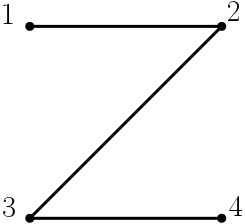
\includegraphics[scale=0.25]{g1}
	\end{subfigure}
\begin{subfigure}[b]{0.16\textwidth}
	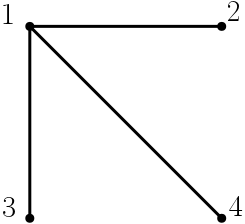
\includegraphics[scale=0.25]{g2}
\end{subfigure}
\begin{subfigure}[b]{0.16\textwidth}
	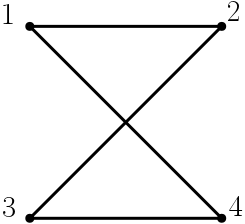
\includegraphics[scale=0.25]{g3}
\end{subfigure}
\begin{subfigure}[b]{0.16\textwidth}
	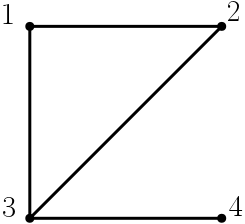
\includegraphics[scale=0.25]{g4}
\end{subfigure}
\begin{subfigure}[b]{0.16\textwidth}
	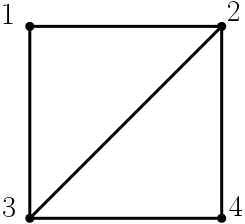
\includegraphics[scale=0.25]{g5}
\end{subfigure}
\begin{subfigure}[b]{0.16\textwidth}
	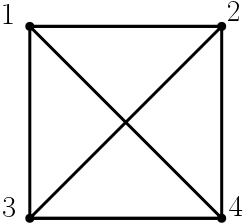
\includegraphics[scale=0.25]{g6}
\end{subfigure}\\
\vspace{0.3cm}
\begin{subfigure}[b]{0.16\textwidth}
	\centering
	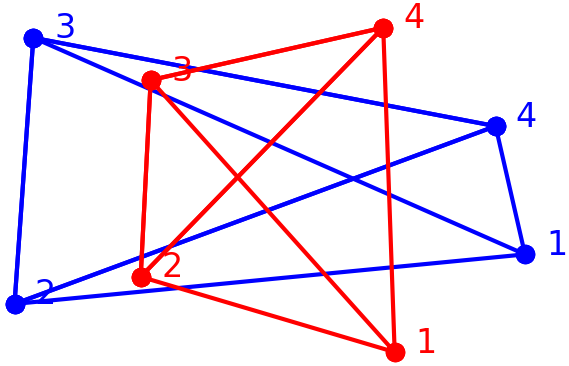
\includegraphics[scale=0.3]{g1_comb}
\end{subfigure}
\begin{subfigure}[b]{0.16\textwidth}
	\centering
	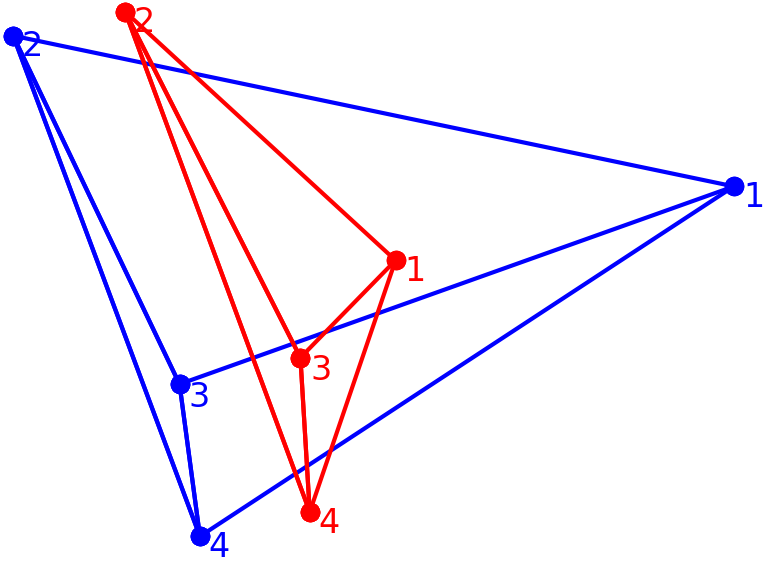
\includegraphics[scale=0.3]{g2_comb}
\end{subfigure}
\begin{subfigure}[b]{0.16\textwidth}
	\centering
	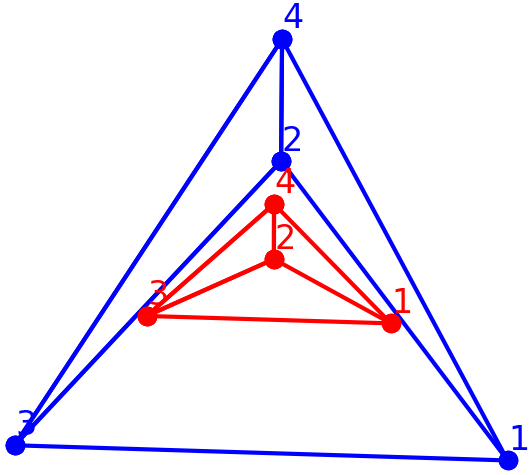
\includegraphics[scale=0.3]{g3_comb}
\end{subfigure}
\begin{subfigure}[b]{0.16\textwidth}
	\centering
	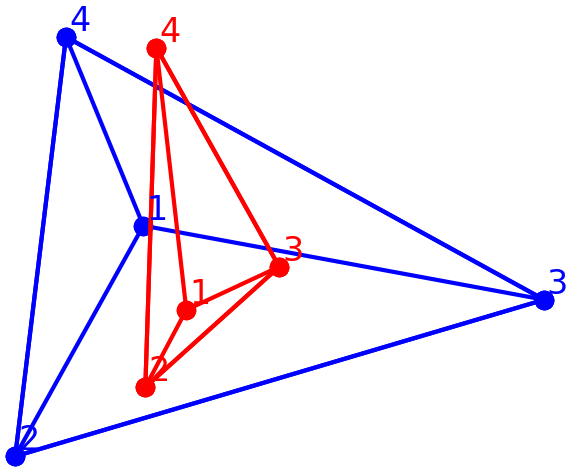
\includegraphics[scale=0.3]{g4_comb}
\end{subfigure}
\begin{subfigure}[b]{0.16\textwidth}
	\centering
	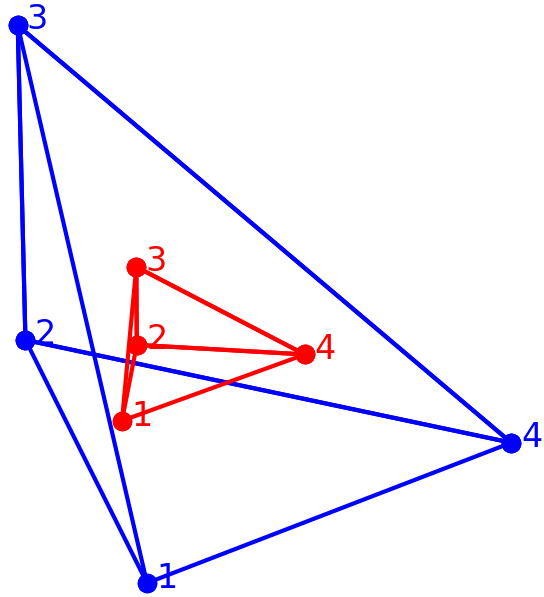
\includegraphics[scale=0.3]{g5_comb}
\end{subfigure}
\begin{subfigure}[b]{0.16\textwidth}
	\centering
	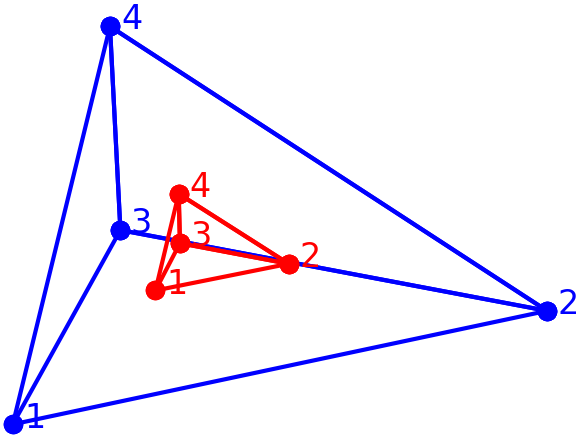
\includegraphics[scale=0.3]{g6_comb}
\end{subfigure}\\
\vspace{0.3cm}
\begin{subfigure}[b]{0.16\textwidth}
	\centering
	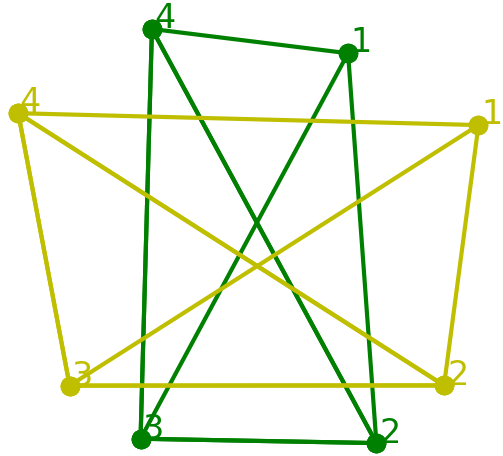
\includegraphics[scale=0.3]{g1_norm}
\end{subfigure}
\begin{subfigure}[b]{0.16\textwidth}
	\centering
	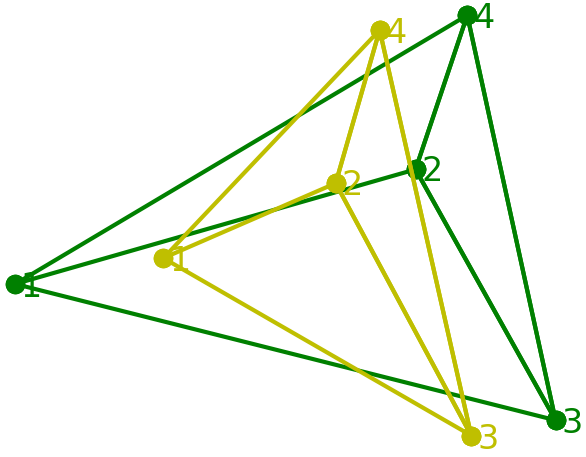
\includegraphics[scale=0.3]{g2_norm}
\end{subfigure}
\begin{subfigure}[b]{0.16\textwidth}
	\centering
	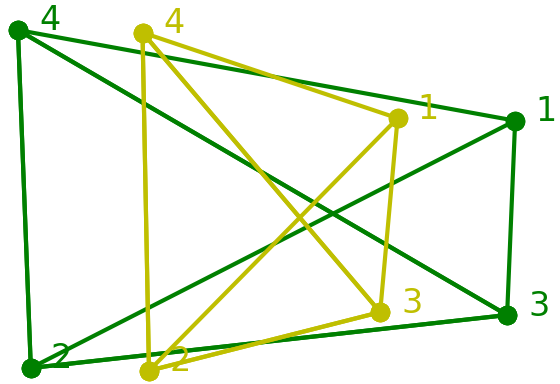
\includegraphics[scale=0.3]{g3_norm}
\end{subfigure}
\begin{subfigure}[b]{0.16\textwidth}
	\centering
	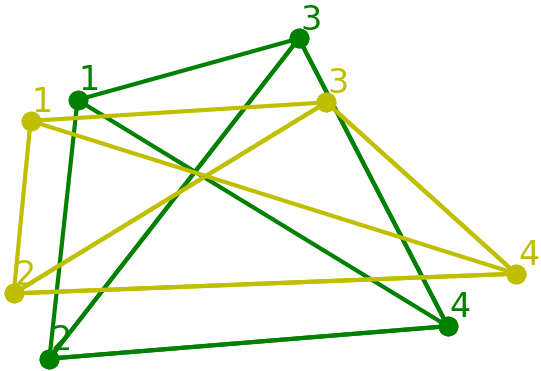
\includegraphics[scale=0.3]{g4_norm}
\end{subfigure}
\begin{subfigure}[b]{0.16\textwidth}
	\centering
	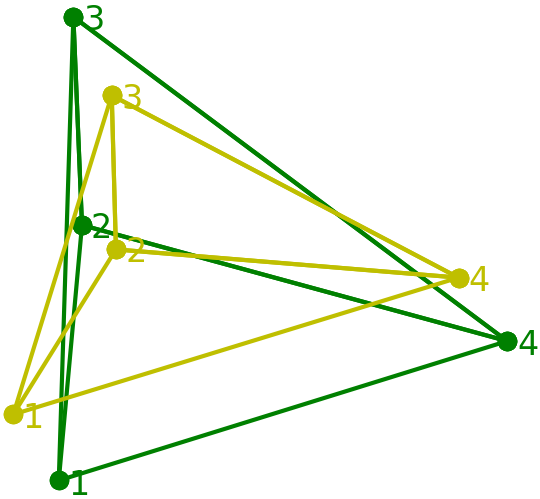
\includegraphics[scale=0.3]{g5_norm}
\end{subfigure}
\begin{subfigure}[b]{0.16\textwidth}
	\centering
	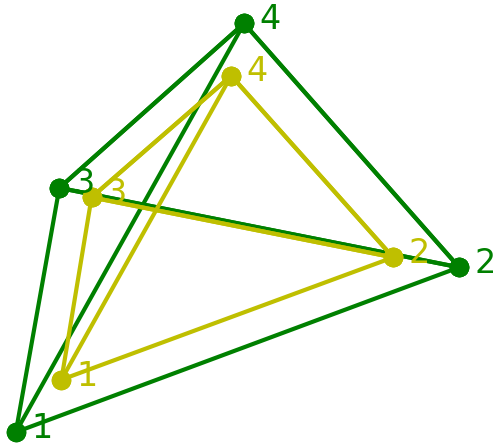
\includegraphics[scale=0.3]{g6_norm}
\end{subfigure}\\

\vspace{0.3cm}
\begin{subfigure}[b]{0.16\textwidth}
	\centering
	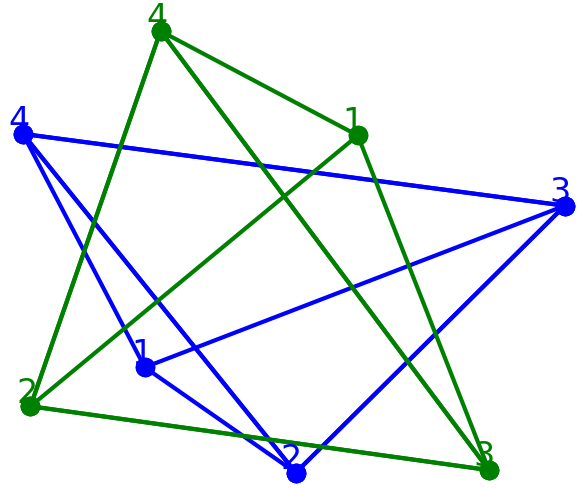
\includegraphics[scale=0.3]{g1_norm_comb}
\end{subfigure}
\begin{subfigure}[b]{0.16\textwidth}
	\centering
	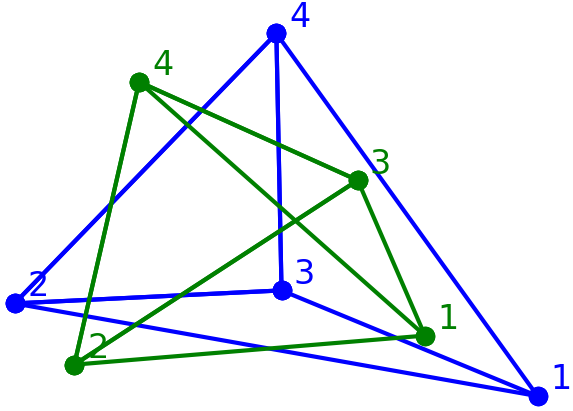
\includegraphics[scale=0.3]{g2_norm_comb}
\end{subfigure}
\begin{subfigure}[b]{0.16\textwidth}
	\centering
	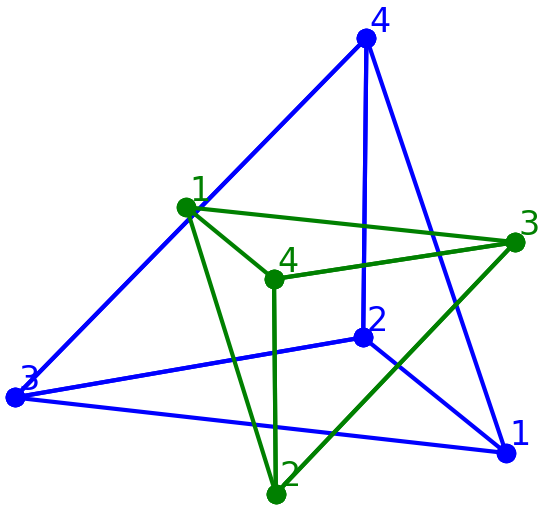
\includegraphics[scale=0.3]{g3_norm_comb}
\end{subfigure}
\begin{subfigure}[b]{0.16\textwidth}
	\centering
	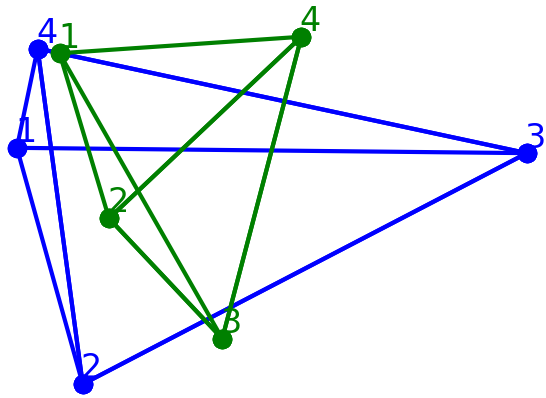
\includegraphics[scale=0.3]{g4_norm_comb}
\end{subfigure}
\begin{subfigure}[b]{0.16\textwidth}
	\centering
	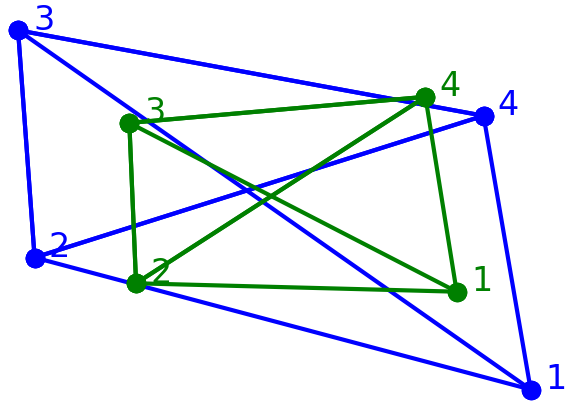
\includegraphics[scale=0.3]{g5_norm_comb}
\end{subfigure}
\begin{subfigure}[b]{0.16\textwidth}
	\centering
	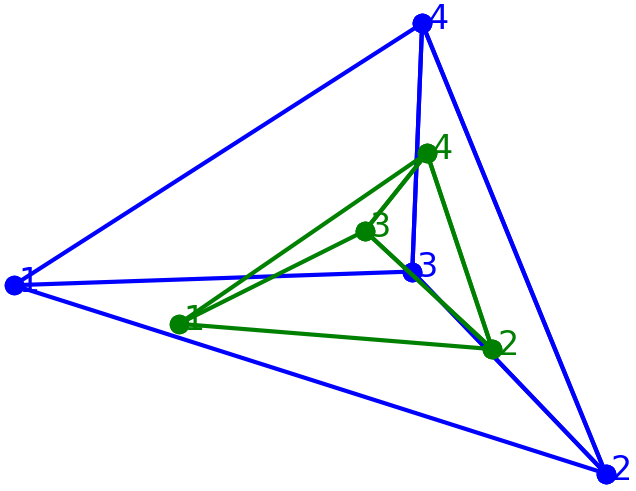
\includegraphics[scale=0.3]{g6_norm_comb}
\end{subfigure}\\
\vspace{0.3cm}
\begin{subfigure}[b]{0.16\textwidth}
	\centering
	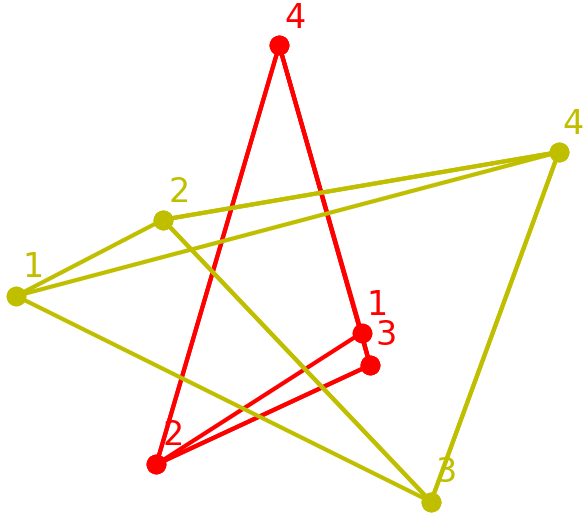
\includegraphics[scale=0.3]{g1_norm_comb_inv}
\end{subfigure}
\begin{subfigure}[b]{0.16\textwidth}
	\centering
	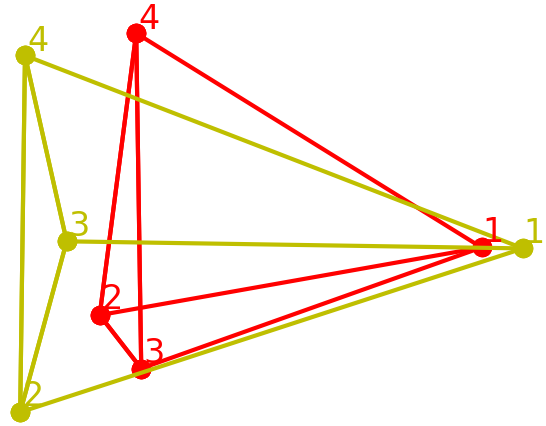
\includegraphics[scale=0.3]{g2_norm_comb_inv}
\end{subfigure}
\begin{subfigure}[b]{0.16\textwidth}
	\centering
	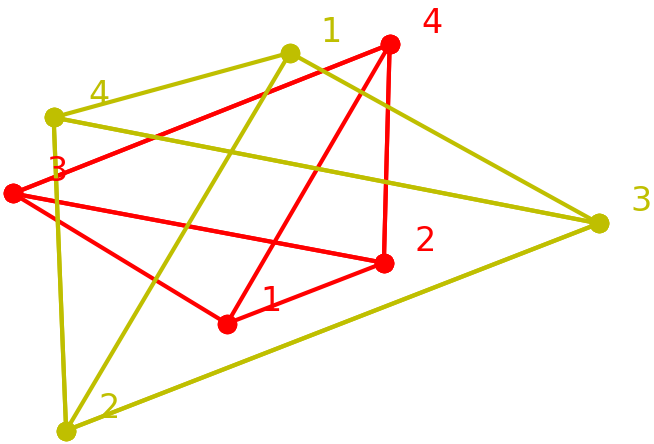
\includegraphics[scale=0.3]{g3_norm_comb_inv}
\end{subfigure}
\begin{subfigure}[b]{0.16\textwidth}
	\centering
	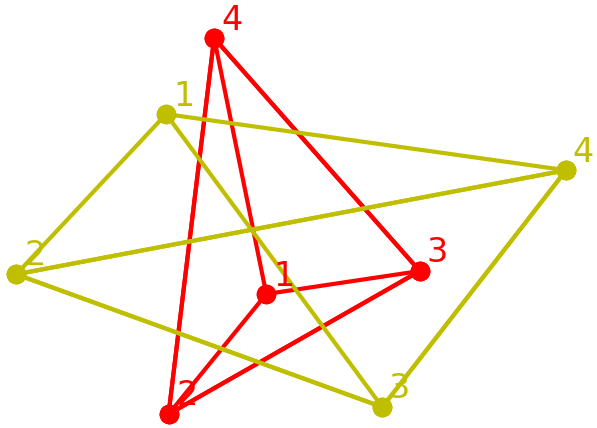
\includegraphics[scale=0.3]{g4_norm_comb_inv}
\end{subfigure}
\begin{subfigure}[b]{0.16\textwidth}
	\centering
	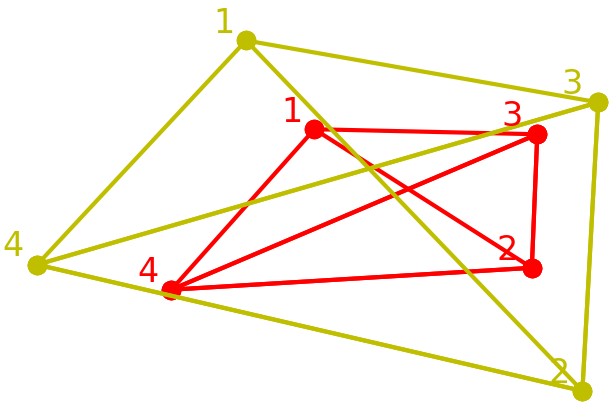
\includegraphics[scale=0.3]{g5_norm_comb_inv}
\end{subfigure}
\begin{subfigure}[b]{0.16\textwidth}
	\centering
	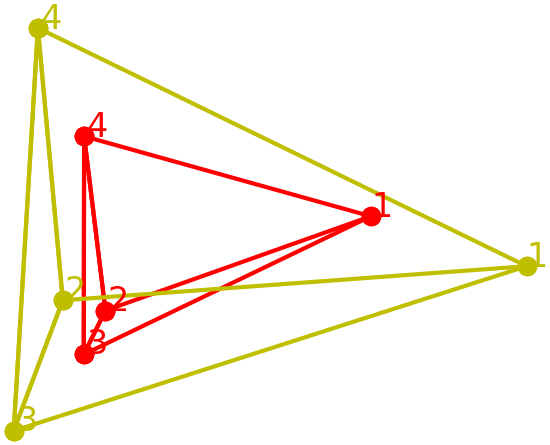
\includegraphics[scale=0.3]{g6_norm_comb_inv}
\end{subfigure}
\caption{The six  unique unweighted  graphs on four vertices, up to isomorphism, and a comparison of all of their simplices. Below each graph in the first row are  its two combinatorial simplices  ($\splx_G$ and $\splx_G^+$), then its two  normalized simplices ($\splxn_G$ and $\splxn_G^+$), then its combinatorial and normalized simplex ($\splx_G$ and $\splxn_G$), followed in  the final  row  by the two inverse simplices ($\splx_G^+$ and $\splxn_G^+$).  The combinatorial simplex and its  inverse are coloured blue and red respectively, and the normalized simplex and its inverse are in green and yellow respectively. The relative size of the the simplices in each subfigure are to scale but the same scale  is not maintained across figures.  }
\label{fig:all_simplices}
\end{figure}







